\section{Test Vorsteuerung}
\begin{figure}[h!]
    \centering
    \begin{subfigure}{0.475\textwidth}
        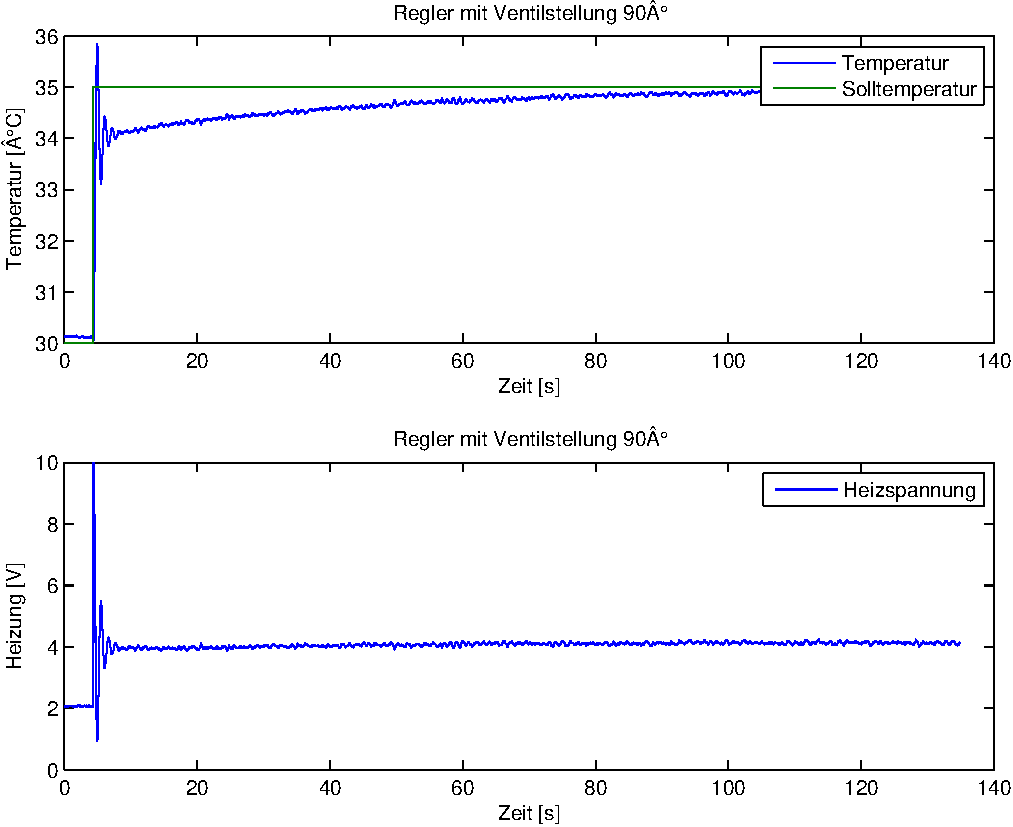
\includegraphics[width=1\textwidth]{11/vorsteuerung_full_plot.pdf}
        \caption{Sprungantwort mit Ventilstellung 90$^\circ$}
        \label{fig:11a}
    \end{subfigure}
    \hfill{}
    \begin{subfigure}{0.475\textwidth}
        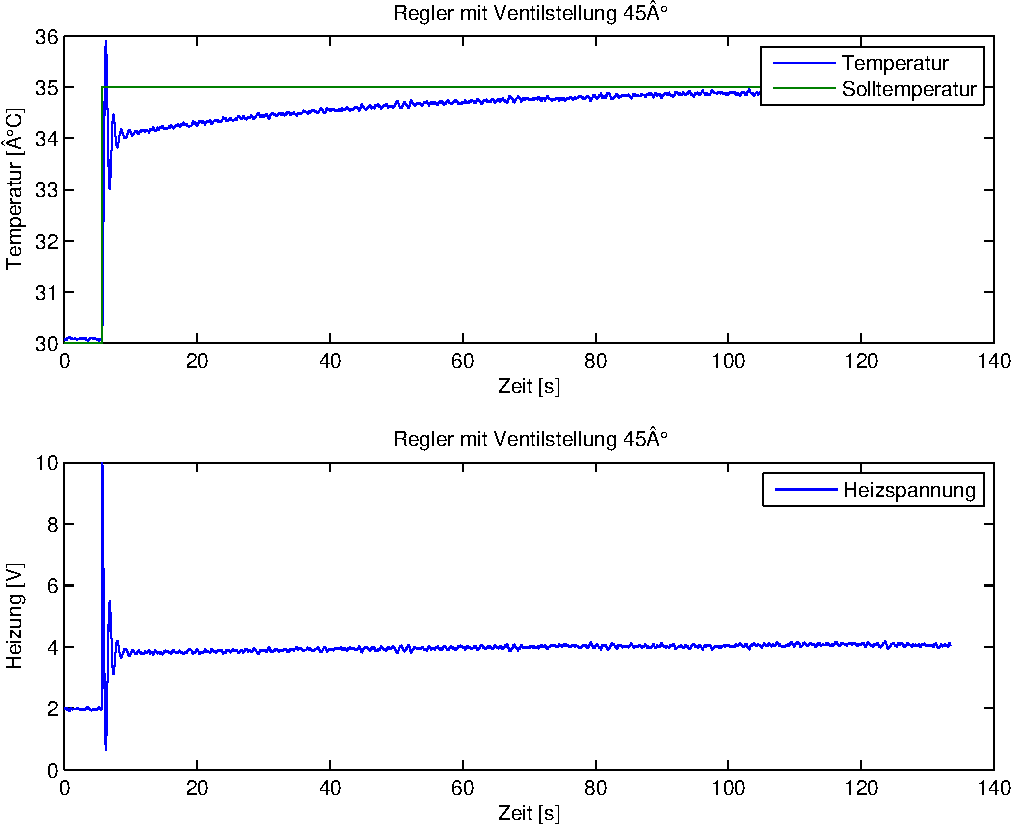
\includegraphics[width=1\textwidth]{11/vorsteuerung_half_plot.pdf}
        \caption{Sprungantwort mit Ventilstellung 45$^\circ$}
        \label{fig:11b}
    \end{subfigure}
\end{figure}
\begin{table}[h!]
	\centering
	\begin{tabular}{l c c c}
		Eigenschaft
			& $\varphi = 90^\circ$
			& $\varphi = 45^\circ$ 
			& Einheit\\
		\hline
		Ausregelzeit ($e < 1\%$)
			& 129
			& 127
            & $\si{\second}$ \\
		Überschwingen
			& 16.92
			& 18.24
			& $\%$
	\end{tabular}
\end{table}
Da die Vorsteuerung nicht mit exakt mit der Strecke übereinstimmt, 
wird der Endwert nicht mit der Vorsteuerung erreicht. Die Differenz muss
der Integrator beisteuern. Da dieser in dieser Konfiguration sehr langsam 
ist, geschieht dieser zweite Ausgleichsvorgang ebenfalls sehr langsam. Die 
Kurve ist dabei der Sprungantwort in \autoref{fig:03a} und \autoref{fig:03b}
ähnlich. 
